%@descr: wzór sprawozdania, raportu lub pracy - nadaje się do przeróbek
%@author: Maciej Komosiński

\documentclass{article} 
\usepackage{polski} %moze wymagac dokonfigurowania latexa, ale jest lepszy niż standardowy babel'owy [polish] 
\usepackage[utf8]{inputenc} 
\usepackage[OT4]{fontenc} 
\usepackage{graphicx,color} %include pdf's (and png's for raster graphics... avoid raster graphics!) 
\usepackage{url} 
\usepackage[pdftex,hyperfootnotes=false,pdfborder={0 0 0}]{hyperref} %za wszystkimi pakietami; pdfborder nie wszedzie tak samo zaimplementowane bo specyfikacja nieprecyzyjna; pod miktex'em po prostu nie widac wtedy ramek
\usepackage{float}

% Zmiana rozmiarów strony tekstu
\addtolength{\voffset}{-1cm}
\addtolength{\hoffset}{-1cm}
\addtolength{\textwidth}{2cm}
\addtolength{\textheight}{2cm}

%bardziej zyciowe parametry sterujace rozmieszczeniem rysunkow
\renewcommand{\topfraction}{.85}
\renewcommand{\bottomfraction}{.7}
\renewcommand{\textfraction}{.15}
\renewcommand{\floatpagefraction}{.66}
\renewcommand{\dbltopfraction}{.66}
\renewcommand{\dblfloatpagefraction}{.66}
\setcounter{topnumber}{9}
\setcounter{bottomnumber}{9}
\setcounter{totalnumber}{20}
\setcounter{dbltopnumber}{9}

% własny bullet list z malymi odstepami
\newenvironment{tightlist}{
\begin{itemize}
  \setlength{\itemsep}{1pt}
  \setlength{\parskip}{0pt}
  \setlength{\parsep}{0pt}}
{\end{itemize}}

%obrazkow szukamy w nastepujacym katalogu:
\graphicspath{{pics/}}



%\title{Sprawozdanie z laboratorium:\\Metaheurystyki i Obliczenia Inspirowane Biologicznie}
%\author{}
%\date{}


\begin{document}

\thispagestyle{empty} %bez numeru strony

\begin{center}
{\large{Sprawozdanie z laboratorium:\\
Przetwarzanie i Rozpoznawanie Obrazów\\
(szablon)}}

\vspace{3ex}

Część III: Segmentacja Semantyczna - Głębokie Uczenie Się

\vspace{3ex}
{\footnotesize\today}

\end{center}


\vspace{10ex}

Prowadzący: dr ~inż. Bartosz Wieloch

\vspace{5ex}

Autorzy:
\begin{tabular}{lllr}
\textbf{Sebastian Firlik} & inf122485 & ISWD & sebastian.firlik@student.put.poznan.pl \\
\textbf{Michał Wójcik} & inf122513 & ISWD & michal.p.wojcik@student.put.poznan.pl \\
\end{tabular}

\vspace{5ex}

Zajęcia środowe, 11:45.

\vspace{35ex}

\noindent Oświadczamy, że niniejsze sprawozdanie zostało przygotowane wyłącznie przez powyższych autorów,
a wszystkie elementy pochodzące z innych źródeł zostały odpowiednio zaznaczone i~są cytowane w bibliografii.  

\newpage



\section{Wstęp}

Zadaniem w niniejszym projekcie było stworzenie programu, który posłużyłby do rozwiązania problemu segmentacji semantycznej. Sam problem segmentacji polega na oddzieleniu od siebie obszarów obrazu, które stanowią odrębne obiekty. Do celu segmentacji wystarczy wykorzystać klasyczne metody przetwarzania obrazów, jak choćby wykrywanie krawędzi, czy też progowaniami na podstawie np. jasności pikseli. Zadanie to jest w większości przypadków dokładnie przestudiowane i rozwiązane, jednakże nie jest to najtrudniejszy możliwy problem, opierający się na rozpoznawaniu osobnych obiektów. Naturalnym rozwinięciem zagadnienia segmentacji jest segmentacja semantyczna. Polega ona na tym, by rozdzielać obiekty, będące w rzeczywistości innymi obiektami. Na przykład: rower składa się z dwóch kół, ramy, siodełka. System nie powinien oddzielać koła od tła, lecz wyodrębniać i nazywać rower jako całość.

To zadanie do niedawna było poza zasięgiem programów komputerowych, jednak obecnie możliwe jest ich rozwiązanie poprzez zastosowanie głębokiego uczenia się. Powstało wiele architektur, pozwalających najpierw na rozwiązanie zadania klasyfikacji, czyli ,,czy na danym obrazku znajduje się pies?'', a następnie ,,gdzie na danym obrazku znajduje się pies?'' czyli właśnie zadanie segmentacji semantycznej. Zasadnicza różnica między powyższymi zadaniami polega na tym, że wyjściem sieci klasyfikującej obrazek jest najczęściej liczba, oznaczająca prawdopodobieństwo, lub etykieta binarna (prawda lub fałsz), natomiast w przypadku \textit{Fully Convolutional Network}, wyjściem jest cały obraz o takiej samej rozdzielczości jak obraz wejściowy, lecz już z naniesionymi barwami, gdzie każde skupisko odpowiada jednemu obiektowi. W tego typu zadaniu należy podać jako źródło wiedzy obrazek wejściowy, lecz oznaczony różnymi skupiskami kolorów, tak, jak twórcy systemu chcą, by ich sieć odpowiadała na dany obraz.

\section{Eksperymenty}

W trakcie tworzenia sieci najefektywniejszej, przeprowadzone zostało bardzo wiele eksperymentów. W tym rozwiązaniu autorzy skupili się na sieci \textit{Fully Convolutional}, której przykładowa architektura pokazana została na rysunku \ref{fig:fcn}.

\begin{figure}[H]
\begin{center}
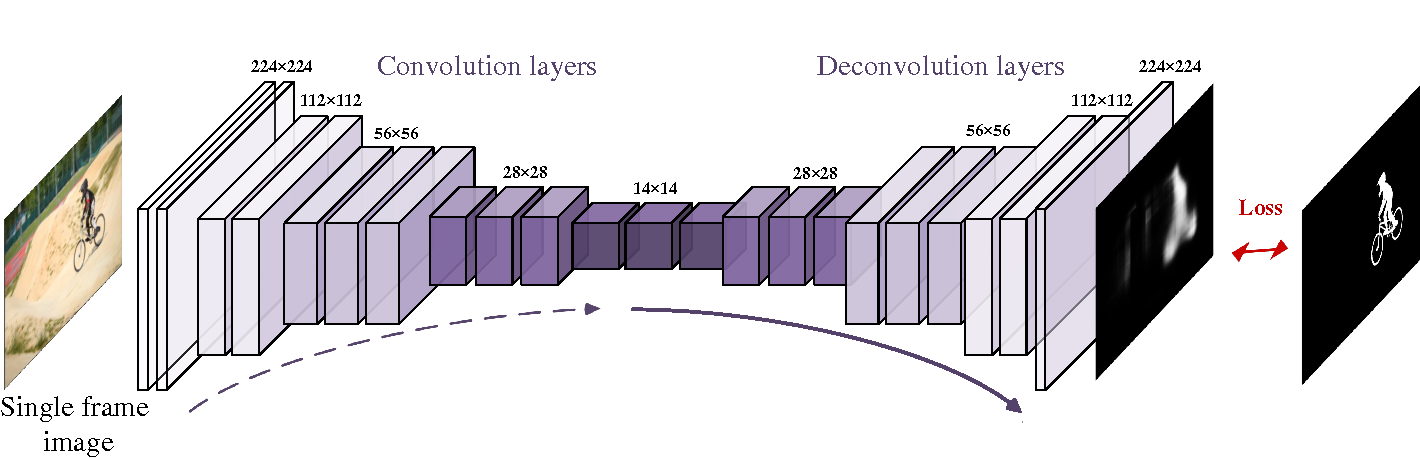
\includegraphics[width=0.9\textwidth]{fcn.png}
\end{center}
\caption{Przykładowa architektura sieci typu Fully Convolutional.}
\label{fig:fcn}
\end{figure}

Sieć tego typu przyjmuje na wejściu obraz, następnie poprzez wielokrotne zastosowanie warstw splotowych, przeplatanych warstwami typu \textit{MaxPooling}, których zadaniem było zmniejszanie odpowiedzi kolejnych zestawów filtrów do coraz mniejszych macierzy. Następnie, po momencie największej kompresji informacji, następuje seria warstw \textit{deconvolutional}, których zadaniem jest powrotna konwersja skompresowanej informacji i odpowiedzi filtrów na obraz o wymiarze dokładnie takim samym jak obraz wejściowy. Funkcja straty ma za zadanie tak kierować nauką sieci, by odpowiedź jak najbardziej przypominała zaetykietowany obraz.

\subsection{Użyte technologie}

Do stworzenia architektury sieci, a także zaimplementowania preprocessingu, funkcji realizującej \textit{data augmentation}, czyli tworzenie syntetycznych przykładów z tych dostępnych posłużył język Python. Został wybrany ze względu na mnogość dostępnych frameworków do głębokiego uczenia się, a także ze względu na łatwość operowania na obrazach, macierzach z wykorzystaniem bibliotek numpy i scikit-image. Początkowo wybrany został framework TensorFlow, jako najpopularniejsze obecnie rozwiązanie, jednak został on porzucony na rzecz Kerasa, korzystającego pod spodem ze środowiska TensorFlow. Zmiana ta nastąpiła, gdyż interfejs programistyczny biblioteki Keras jest przyjaźniejszy niż ten dostępny przy TensorFlow, a do tego powstało bardzo wiele rozwiązań bazujących na tej bibliotece, co pozwalało na dogłębniejsze przestudiowanie potencjalnych architektur i ich skuteczności.

\subsection{Preprocessing i zbiór danych}

Zbiór danych jest dostępny w sieci. Jest to zbiór Massachusetts Roads Dataset, udostępniony przez Uniwersytet w Toronto. Składa się on z około 1100 zdjęć satelitarnych, wraz z odpowiadającą mu etykietą w postaci białych dróg i czarnego tła, czarnych budynków. Po przefiltrowaniu powyższego zbioru zdjęć, zostało 750 zdjęć w dobrej jakości, bez cenzury, z poprawnymi etykietami. Na tym zbiorze zdjęć został zbudowany właściwy zbiór danych. Obrazy dostępne w ramach tego zbioru nie mogły być bezpośrednio podane na wejście sieci, gdyż ich rozdzielczość była zbyt duża i sieć nie potrafiłaby w dopuszczalnym czasie nauczyć się niczego sensownego. W związku z tym została utworzona procedura, która z obrazu wejściowego wycinała losowe wycinki obrazu o rozmiarze 128x128 pikseli. Dzięki temu możliwe było utworzenie dużo większego zbioru danych niż 750 obrazów. Jednakże, przy niektórych eksperymentach problemem okazywała się pamięć i nie dało się dostarczyć tak dużej liczby obrazów wejściowych, jaką funkcja wycinająca była w stanie stworzyć.

\subsection{Utworzone sieci neuronowe}

Eksperymenty rozpoczęły się od testowania możliwości wykorzystania istniejących i sprawdzonych architektur, osiągających bardzo dobre wyniki w podobnych problemach. Pierwsze testy przeprowadzono na sieciach zawierających pięć segmentów, na które składały się dwie lub trzy warstwy konwolucyjne i warstwy MaxPoolingu. Ze względu na 32-krotnie mniejszy rozmiar takiego obrazu, konieczne było zastosowanie na końcu warstwy realizującej operację Upsamplingu, która aproksymowała brakujące wartości pikseli, powstałe na skutek zwiększenia rozdzielczości obrazu. Rozwiązanie to było testowane z różnymi wartościami parametrów takich jak rozmiar batcha, współczynnik uczenia i liczności neuronów na poszczególnych warstwach. Modyfikacji ulegała również używana w celu nauki funkcja straty. Testy tak zaprojektowanych sieci dawały jednak bardzo słabe wyniki, prawdopodobnie ze względu na dużą utratę informacji i brak możliwości wyrażenia zdobytej wiedzy w wyniku operacji Upsamplingu.

Kolejna próba oparta była o rozszerzenie pierwotnej koncepcji o stopniowe powiększanie rozdzielczości obrazu naprzemian ze splotami obrazów z tymi uzyskanymi na wcześniejszych warstwach konwolucyjnych. Ta koncepcja wydawała się bardziej skuteczna, jednak w procesie nauki postępy zachodziły bardzo powoli ze względu na bardzo dużą liczbę wag.

\begin{figure}[H]
\begin{center}
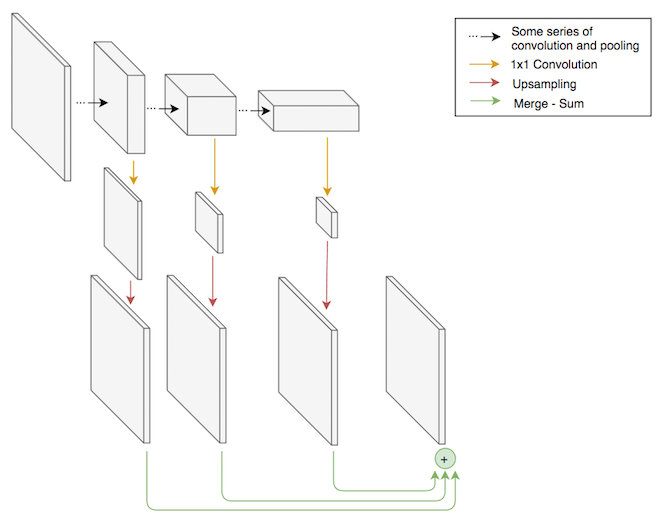
\includegraphics[width=0.9\textwidth]{fcn_modified.png}
\end{center}
\caption{Zastosowana architektura sieci FCN}
\label{fig:mod}
\end{figure}

Dobrym kompromisem pomiędzy powyższymi podejściami okazała się koncepcja wykorzystania wyników uzyskanych z każdego wcześniejszego segmentu, poddaniu ich konwolucji i Upsamplingowi do oczekiwanego, finalnego rozmiaru, a następnie konkatenację i splotu tak uzyskanych obrazów. Koncepcja widoczna jest na rysunku \ref{fig:mod}. Rozwiązanie to pozwalało na lepszą reprezentację uzyskanej wiedzy w połączeniu ze stosunkowo niskimi kosztami obliczeniowymi w procesie nauki, dzięki czemu sieć zaczęła osiągać dobre wyniki.

Poczyniono również wiele prób wyboru odpowiedniej funkcji celu do postawionego problemu. Badania rozpoczęto od koncepcji opartej o minimalizację błędu średniokwadratowego,  a następnie próbie wykorzystania miary entropii krzyżowej, która jest popularną metodą w problemach segmentacji semantycznej zorientowanej na wiele klas. Ostatecznie zdecydowano się na Współczynnik Dice'a, wyrażający się wzorem

\[ Dice(A, B) = \frac{2 \cdot C + 1}{A + B + 1}\]

gdzie licznik to podwojona suma iloczynów wartości poszczególnych pikseli w dwóch obrazach, a mianownik jest sumą wartości pikseli w obu obrazach. W przypadku obrazów, których wartości pikseli wyrażają prawdopodobieństwo przynależności do danej klasy, współczynnik ten przyjmuje wartość 1 dla dwóch tożsamych obrazów i wartość 0 dla obrazów nie posiadających żadnej części wspólnej. Dodanie wartości 1 w liczniku i mianowniku nieznacznie modyfikuje wartość funkcji, ale pozwala zagwarantować niezerowy mianownik i pozostawić przeciwdziedzinę funkcji w zakresie $[0 ; 1]$. W takim wypadku konieczne jest zagwarantowanie również, że obraz wychodzący z sieci neuronowej będzie również wyrażał prawdopodobieństwo klasyfikacji i przyjmował wartości z takiego samego zakresu. W tym celu na końcu sieci dodano warstwę z sigmoidalną funkcją aktywacji, zaś zastosowaną funkcją celu była różnica pomiędzy wartością funkcji, a wartością 1, czyli idealnym odtworzeniem wzorca.

\section{Wyniki}

Po każdej epoce nauki, sieć była zapisywana do pliku, dzięki czemu w trakcie tego procesu mogliśmy na bieżąco monitorować jej wyniki na zbiorze walidującym i testowym. Co kilka epok (od 1 do 5) tworzony był nowy zbiór uczący, zawierający zwykle po 32 wycinki z 5 obrazów z dostępnego zbioru. Sieć była uczona w tej sposób przez około 1000 epok. Po procesie nauki, w celu zwiększenia jakości rozwiązania, podjęto próbę zastosowania postprocessingu, opartego o operacje morfologiczne i progowanie obrazu. Pomimo zastosowania kilku operacji otwarcia i domknięcia, na obrazach wyjściowych pozostawały niewielkie szumy. Aby je usunąć, każdy z obrazów był dzielony na spójne obszary. Następnie podjęto próbę mającą na celu maksymalizację współczynnika Intersection over Union, który jest bardzo podobny do współczynnika Dice'a, ale możliwy w zastosowaniu do dwóch binarnych obrazów, stąd konieczność wcześniejszego progowania. Poprzez testowanie kolejnych wartości progu rozmiaru spójnych obszarów, mierzonych w liczności pikseli, małe obszary były zerowane, co nieznacznie podniosło jakość ostatecznego rozwiązania.

Do odtworzenia obrazu o pierwotnej rozdzielczości, konieczne było podzielenie go na mniejsze fragmenty, przetworzenie przez sieć, a następnie połączenie fragmentów w całość. Najlepiej sprawdziło się przesuwanie okna o rozmiarze obrazu wejściowego sieci (128 x 128 pikseli) na obrazie wejściowym o wartość parametru split, który ustalony został na 49, ze względu na co najmniej jednokrotną klasyfikację każdego z pikseli przy zachowaniu rozsądnego czasu przetwarzania. W przypadku kilkukrotnego poddaniu działaniu sieci danego piksela, wynik prawdopodobieństwa jego klasyfikacji był uśredniany. Po połączeniu ze sobą wszystkich fragmentów, obraz poddawany był wyżej opisanemu postprocessingowi.

\begin{figure}[H]
\begin{center}
\includegraphics[width=0.9\textwidth]{example.png}
\end{center}
\caption{Obraz wejściowy, klasyfikacja wzorcowa po lewej i uzyskana przez algorytm po prawej stronie.}
\label{fig:example}
\end{figure}

Ostatecznie, zastosowanie takiej procedury na całym zbiorze testowym skutkowało osiągnięciem wartości parametru IoU na poziomie ponad 0.47 przy porównaniu parami wzorców i obrazów wyjściowych po przetworzeniu przez sieć i postprocessingu. Przykładowy wynik działania sieci w porównaniu z oczekiwanym wynikiem i obrazem wejściowym widoczny jest na rysunku \ref{fig:example}.

\section{Podsumowanie}

Projekt pozwolił nam na pogłębienie wiedzy z zakresu budowy i działania sieci neuronowych, w szczególności w wersji konwolucyjnej. Poszerzyliśmy wiedzę z zakresu sieci sprawdzających się w zadaniach segmentacji semantycznej, a więc sieci typu Fully Convolutional Network. Nauczyliśmy się także konstruowania sieci przy pomocy narzędzi dostępnych w bibliotekach języka Python. Dowiedzieliśmy się w jaki sposób można projektować i modyfikować topologię, przygotować zbiór uczący i dostosować parametry takie jak funkcje aktywacji neuronów do wybranej funkcji celu.

\clearpage %pozwol LaTeX'owi umiescic zaległe rysunki od razu tutaj -- "uwalnia" nagromadzone zaległości, dzięki temu nie wylądują na końcu dokumentu





%%%%%%%%%%%%%%%% literatura %%%%%%%%%%%%%%%%

\bibliography{sprawozd}
\bibliographystyle{plainurl}


\end{document}
